%-----------------------------------------------------------------------------%
%Packages%
\documentclass[12pt, a4paper, titlepage]{article}
\usepackage{amsmath, amsfonts, listings, amssymb, mathtools, amsthm} %Mathematical Expressions package
\usepackage{mathtools}
\usepackage[usenames, dvipsnames]{color} %Color naming packages
\usepackage{geometry}
\usepackage{float}
\usepackage{verbatim} %for code
\usepackage[pdftex]{graphics}
\usepackage{hyperref}
\usepackage{cleveref}
\usepackage{tikz}
\usepackage[nottoc]{tocbibind}
\usepackage{caption}
\usepackage{subcaption}
\usepackage{fancyhdr}
\usepackage{array}

\usetikzlibrary{arrows,shapes}

%Graphis Extensions
\DeclareGraphicsExtensions{.png, .jpg}
\parindent 0pt

% Predefined things such as commands, etc.
\newcommand{\FIXME}{{\bf FIXME}}
% Drawings of frames

\tikzstyle{vertex}=[circle,fill=black!25,minimum size=20pt,inner sep=0pt]
\tikzstyle{selected vertex} = [vertex, fill=red!24]
\tikzstyle{edge} = [draw,thick,->]
\tikzstyle{weight} = [font=\small]

\setlength{\headheight}{15.2pt}
\pagestyle{fancy}

\fancyhf[FC]{\thepage}
\fancyhf[HL]{Edwin Richard Yucheng Tay, 20529864}
\fancyhf[HR]{CITS5502 Assignment One}

%-----------------------------------------------------------------------------%
%Document%

\title{CITS5502: Software Processes Taxonomy}
\author{Edwin Richard Yucheng Tay, 20529864 \\
University of Western Australia \\
email: taye03@student.uwa.edu.au }

\date{\today}

\begin{document}

\maketitle

\begin{abstract}
TODO BY 1030 14th AUGUST 2013
\end{abstract}


\tableofcontents

\section{Introduction --- TODO by 0930 14th August 2013} \label{introduction}

In today's software development industry, the methodology of software development is fractured
between multiple processes.
Some companies use an ``agile" methodology, iteratively developing ideas and prototyping their
products \FIXME. %need a citation
Others develop according to the traditional Software Development Lifecycle (SDLC) models, requiring
extensive documentation and requirements before beginning software development \FIXME.\\
\\
These are confusing categorisations, and within each are further sub-models, such as \FIXME
%citations below
\begin{itemize}
	\item ``Spiral"
	\item ``Extreme Programming"
	\item ``Prototyping"
	\item ``V-Model"
\end{itemize}
Depending on what project, some development processes are not even suitable for some software
projects and it is thus desirable to gauge how suitable one process is compared to another.\\
\\
However, each is denoted in its own format and style, making identification and classification of processes a
confusing task \FIXME. %add diagrams
Comparisons about the strengths and weaknesses of each process and their suitability to fulfill a
project are thus difficult to conceive.\\
\\
We will resolve these difficulties in by introducing a simple flow-chart based notation with some
relations to UML-activity diagrams.
This standardised notation will be further augmented with a descriptive aid and translation to a
C-style imperative language.\\
\\
We construct a taxonomy based on the distinguishing features between a set of software development
processes.
Our taxonomy will have two aims
\begin{enumerate}
	\item given a software development process, which known software development process does it most
	resemble?
	\item given a description of informal software requirements, which known software development
	process would be suitable for its development?
\end{enumerate}

Finally, we present an analysis of the taxonomy and significant or interesting results we have
found during through the taxonomy.
We discuss what makes our taxonomy and classification system worthwhile for usage and present
conjectures about improving classification methods.

\section{Software Process Notation --- TODO by 0000 13th August 2013} \label{notation}

In Section \ref{introduction}, we briefly discussed the idea of classifying and comparing models.
As we further noted, the different process descriptions make classification and comparison of
development processes difficult.
Thus, we introduce a standardised notation that will allow us to describe and discuss software
processes in an unambiguous manner.\\
\\
To a reader interested in the notation used throughout the paper, we direct them
to \FIXME which summarises the graphical notations we have
designed.
It gives the natural language meaning and semantics of each of the symbols we employ.\\
\\
Otherwise, this chapter introduces our graphical notation by justifying each symbol we
use.
We draw inspiration from UML Activity Diagrams \cite{Dumas01umlactivity,BellUMLBasics}, as well as
the notation Woodings describes in \ref{Woodings2013Tut1}.
We discuss the design and ideas behind our notation, and why we believe it is a
good notation system.
\subsection{Notation}

In \cite{fuggetta2000software} we define a process as
\begin{quote}
A software process can be defined as the coherent set of policies, organizational structures,
	technologies, procedures, and artifacts that are needed to conceive, develop, deploy, and maintain
	a software product.
\end{quote}

From this definition, we can note that we must be able to at least denote four things
\begin{itemize}
	\item a point at which the set of policies and technologies should begin deployment
	\item a point at which the policies and technologies should cease operation on the software
	product development
	\item sub-tasks to arbitrarily divide the component procedures of a process into as fine detail as
	is necessary
	\item inputs and outputs which are the artifacts used within a software development process
\end{itemize}

We first introduce the entry and exit points of a process; these are the points where it starts and
ends.

\begin{figure}[h!]
\centering
\begin{subfigure}[b]{.45\textwidth}
\centering

\includegraphics[scale=0.6]{media/Entry}
\caption{The entry point in the program.}
\label{entryFigure}
\end{subfigure}
~
\begin{subfigure}[b]{.45\textwidth}
\centering

\includegraphics[scale=0.6]{media/Exit}
\caption{The exit point of the program.}
\label{exitFigure}
\end{subfigure}
\caption{Here, we show our notation for the entry and exit points of a process.
Note that it is quite similar to notation in \ref{Dumas01umlactivity} for
  signifying where a process begins and ends.}
\label{entryExitFigure}
\end{figure}

Without knowing where we start and end, our process is a never-ending sequence of tasks, which
either has no recognisable place to start or no point to recognise the software product as
``finished".
This is counter-intuitive to the purpose of a process which is to construct a software product.\\
\\
Next, we define a sub-task.
As we noted in our previous definition, there are sub-procedures which make up our process.

\begin{figure}[h!]
\centering
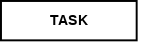
\includegraphics[scale=0.6]{media/Task}
\caption{A single task of a process.}
\label{taskFigure}
\end{figure}

In \cite{Woodings2013Tut1}, Woodings comments on the need to break down a
process into tasks.
A process that consists of a single task is pointless, as it offers no new
insights into the innards and comparability of a process.\\
\\
Thus, a single task must act on {\em something}, and as a result of its actions
it must produce something different.
To denote dependencies upon inputs or other tasks, we use arrows, whilst we denote tangible outputs
from a task with a circle.

\begin{figure}[h!]
\centering
\begin{subfigure}[b]{.45\textwidth}
\centering
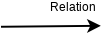
\includegraphics[scale=0.6]{media/Dependency}
\caption{The arrow denotes a dependency of one task on another. As an example, suppose $A \to B$.
	Then $B$ is dependent on $A$.
We can add further detail to this dependency by labelling the relation.}
\label{depFigure}
\end{subfigure}
~
\begin{subfigure}[b]{.45\textwidth}
\centering
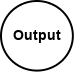
\includegraphics[scale=0.6]{media/Output}
\caption{This circle denotes the output from a task, but also the input to another task. It
is logical that each output is used as the input of {\em some} point in the process (including the
		exit point), otherwise the output itself has no usage.}
\label{outputFigure}
\end{subfigure}
\caption{An arrow will show dependency and a circle shows the output of a task,
which also denotes the input for some point in the process.} \label{depOutFigure}
\end{figure}

Note that we have said that \ref{outputFigure} denotes either an input or an
output.
We note that although an output must implicitly be an output to some other
process point, inputs need not necessarily be generated from a task.
Similarly, we do not make the claim that all tasks require inputs, only that
they must generate some output.\\
\\
Processes may branch at certain points due to needing to make a decision on the conditions of the
process and the appropriate path the process should take to complete development.
We will call these ``decision points".
At other times, tasks can be parallelised between members of the software development team.

\begin{figure}[h!]
\centering
\begin{subfigure}[b]{.45\textwidth}
\centering

\includegraphics[scale=0.6]{media/Parallelised}
\caption{The above notation symbolises that multiple tasks should begin occurring in parallel (that
		is, simultaneously).}
\label{parFigure}
\end{subfigure}
~
\begin{subfigure}[b]{.45\textwidth}
\centering
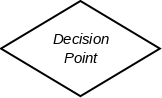
\includegraphics[scale=0.6]{media/Branching}
\caption{The following is a decision point, where multiple paths can emerge from this single point.}
\label{branFigure}
\end{subfigure}
\end{figure}

\pagebreak %TODO: Check if pagebreak is good idea

Finally, we pay a special attention to the verification process.
Verification that a task is correct and its outputs meet the requirements and standards expected by a client
and other software maintainers is, in itself a process.
We separate our notation of verification to thus distinguish it as a ``shadow" or ``reflection"
procedure of a task (or sequence of tasks).

\begin{figure}[h!]
\centering
\begin{subfigure}[b]{.45\textwidth}
\centering

\includegraphics[scale=0.6]{media/BeginVerification}
\end{subfigure}
~
\begin{subfigure}[b]{.45\textwidth}
\centering
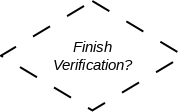
\includegraphics[scale=0.6]{media/EndVerification}
\end{subfigure}
\caption{Here, verification is treated as its own subprocess. The notation has the same meaning as
	\ref{taskFigure} or \ref{branFigure}, except restricted to the verification process.
	However, its dotted-line distinction is
	two-fold; it is the ``shadow" process to ensure that a task has been completed correctly, but is
		also treated in an ad-hoc and almost ``optional" manner by organisations.
		Thus it is not a ``solid" or ``defined" process like \ref{taskFigure} or \ref{branFigure}.}
\label{verification}
\end{figure}

\subsection{Design}

The Object Modelling Group (OMG) specifies in \ref{bpmnfaq} that their Business Process Modelling Notation
specifies ``the sequence of processes and messages" that are passed during a related set of
activities.\\
\\
More importantly, \ref{bpmnfaq} states that a business user or manager ``should be able to easily
understand a BPMN business process diagram."
Conversely, a process implementer or reviewer ``should be able to adorn BPMN with further detail to
represent the process in a physical implementation."\\
\\
We are converging on a set of criteria with which to judge a notation and argue for its usefulness,
but as of yet our quotes have not explicitly stated what we want out of a notation.
Woodings (in \ref{Woodings2013Tut1}) extends the implications stated by the OMG, by listing three criteria for a notation
\begin{enumerate}
	\item simple, or easily understandable by a reader \label{simpleNot}
	\item detailed, and thus conveying enough meaning to a reader to implement and follow
	a process \label{detailedNot}
	\item complete, shows all essential features of a process \label{completeNot}
\end{enumerate}

We will address our notation with respect to each of the three criteria separately.
Firstly, we note that our notation is limited, with only nine different symbols.
Each symbol within our notation has a well-defined semantics, and thus the process notation has a
clear and understandable meaning.
In this way, we believe that criterion \ref{simpleNot} is fulfilled.\\
\\
Next, we address criterion \ref{detailedNot}.
We noted that for a software development process $P$, we wished to break it into a set of tasks
$T_1, T_2, \ldots, T_n$.
We also noted that a process $P$ always outputted or delivered some kind of output, which is akin to
a task as defined above.\\
\\
Then there is nothing that stops us from, for a $T_k$, performing the same analysis and breaking
$T_k$ into a set of subtasks $T'_1, T'_2, \ldots, T'_{n'}$.
A simple inductive argument will show that we can break down our process to an arbitrarily fine
granularity and thereby add as much detail as is necessary to our notation.
In this way, we can fulfill critertion \ref{detailedNot}.\\
\\
Finally, we address \ref{completeNot}.
We must show that our notation captures all essential features of a process.
Our notation uses natural language to describe tasks and dependencies in arbitrarily detail.
In addition, we cover tasks which branch or iterate, feedback and parallelisation of tasks.
It is difficult to conceive how any feature cannot thus be captured by the flexibility of natural
language and the given structural constructs we already have.\\
\\
In having a simple, yet arbitrarily detailed (and thus powerful) notation, we have a standard method
for treating processes.
We can now really begin to compare and contrast different software development processes.

\subsection{Summary}

We present a summarised table of our operators.

\begin{table}

\end{table}

\section{Software Process Representations} \label{diagrams}

In the following section, we use our notation to depict 

\subsection{Software Development Lifecycle (SDLC) and its variants}
Royce first introduced and formalised the SDLC in
\cite{Royce:1987:MDL:41765.41801}.
He was quick to criticise the SDLC as a software development methodology, and pointed out its flaws
and inflexibility to handle software development.
In particular, he noted that its roots were in engineering and other physicals sciences, and the
nature of software meant that it was ineffective and caused much work to be redundantly repeated.\\
\\
This model is commonly known as a ``Waterfall" lifecycle development model, due to the way
activities cascaded in the original model.
We reproduce his diagrams in our own notation as follows.
In Figure \ref{waterfallRoyceOne}, we show our interpretation of Royce's unmodified waterfall model.

\begin{figure}[ht!]
	\centering
	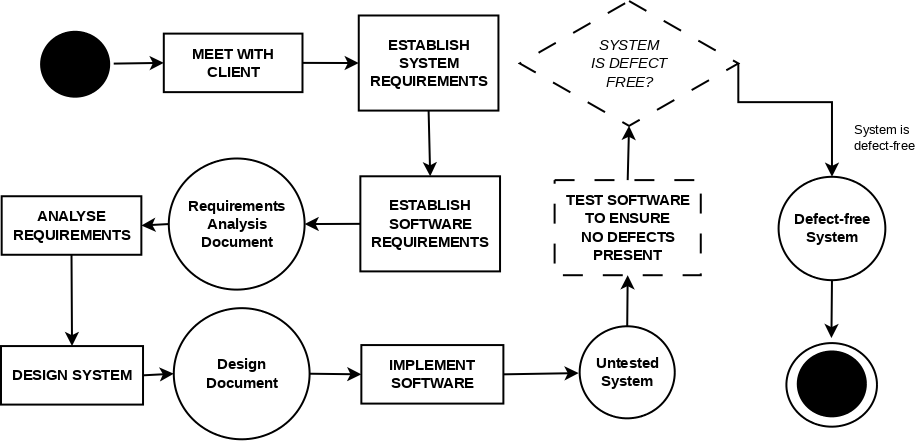
\includegraphics[scale=0.3]{media/WaterfallRoyceOne}
	\caption{Royce's original waterfall model. This is the theoretical way that the SDLC works.}
	\label{waterfallRoyceOne}
\end{figure}

Royce points out the flaws in this model, by revealing that we actually make mistakes and
assumptions when we gather requirements, design a system or implement a system in code.
These assumptions are actually defects that propagate throughout a system, and we are forced to
backtrack to earlier tasks and repeat these tasks in order to fix them.
This can involve backtracking from implementing a feature, to checking how it was designed, to
regathering requirements for this feature upon realising that a client does not actually need that
feature.
Royce claimed this backtracking was quite a significant delay and waste of resources, and we
illustrate his point in our notation in Figure \ref{waterfallRoyceTwo}.

\begin{figure}[ht!]
	\centering
	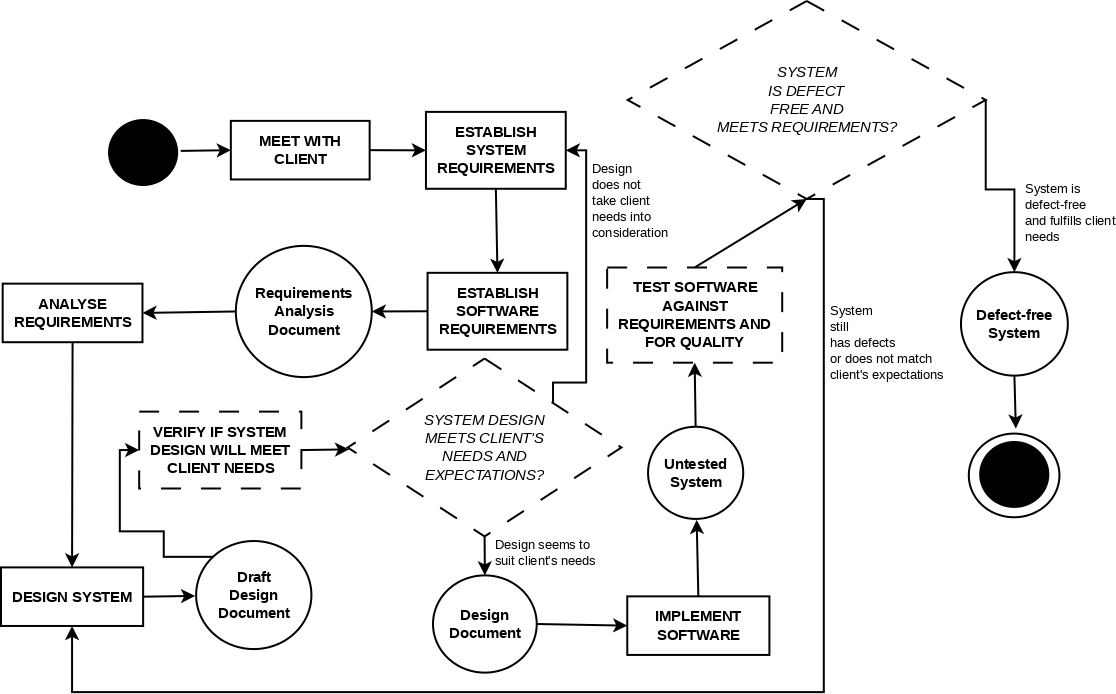
\includegraphics[scale=0.3]{media/WaterfallRoyceTwo}
	\caption{Royce claims that this modified waterfall method was inefficient and caused unnecessary
		backtracking, but that in 1987 it was the current mode of software production.}
	\label{waterfallRoyceTwo}
\end{figure}

Royce suggests an alternative model, which involves iterations and backtracking between stages to
minimise the repeated work.
This recognition that some sort of iteration is necessary to develop good software is perhaps the
beginning of some of the iterative models that we later discuss.
We show Royce's final model in our own notation in \ref{waterfallRoyceThree}, with a heavy emphasis
on verification between each stage to dictate the backtracking.

\pagebreak

\begin{figure}
	\centering
	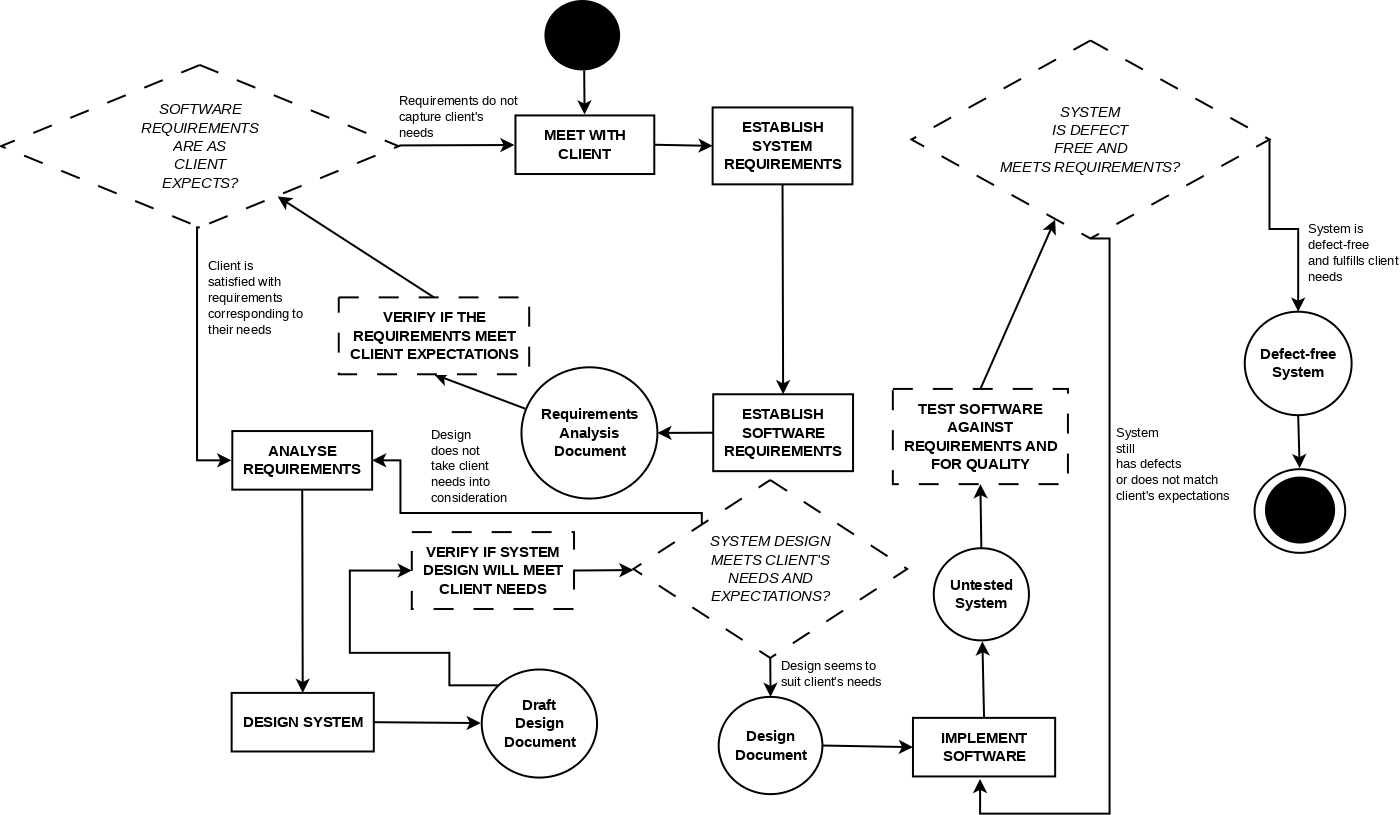
\includegraphics[angle=90,scale=0.3]{media/WaterfallRoyceThree}
	\caption{Royce's final waterfall model resolves the repetition in process work by increasing the
		verification and iteration between stages. We replicate this in our own notation.}
	\label{waterfallRoyceThree}
\end{figure}

\subsection{Spiral}
The Spiral model is introduced by Boehm in \cite{Boehm:1986:SMS:12944.12948}.
It attempts to address some of the weaknesses revealed in SDLC.
It has more concepts of verification and risk analysis built into it.
We show the Spiral model, after it has been unrolled from its original form, in Figure
\ref{Spiral}.\\
\\

\begin{figure}
	\centering
	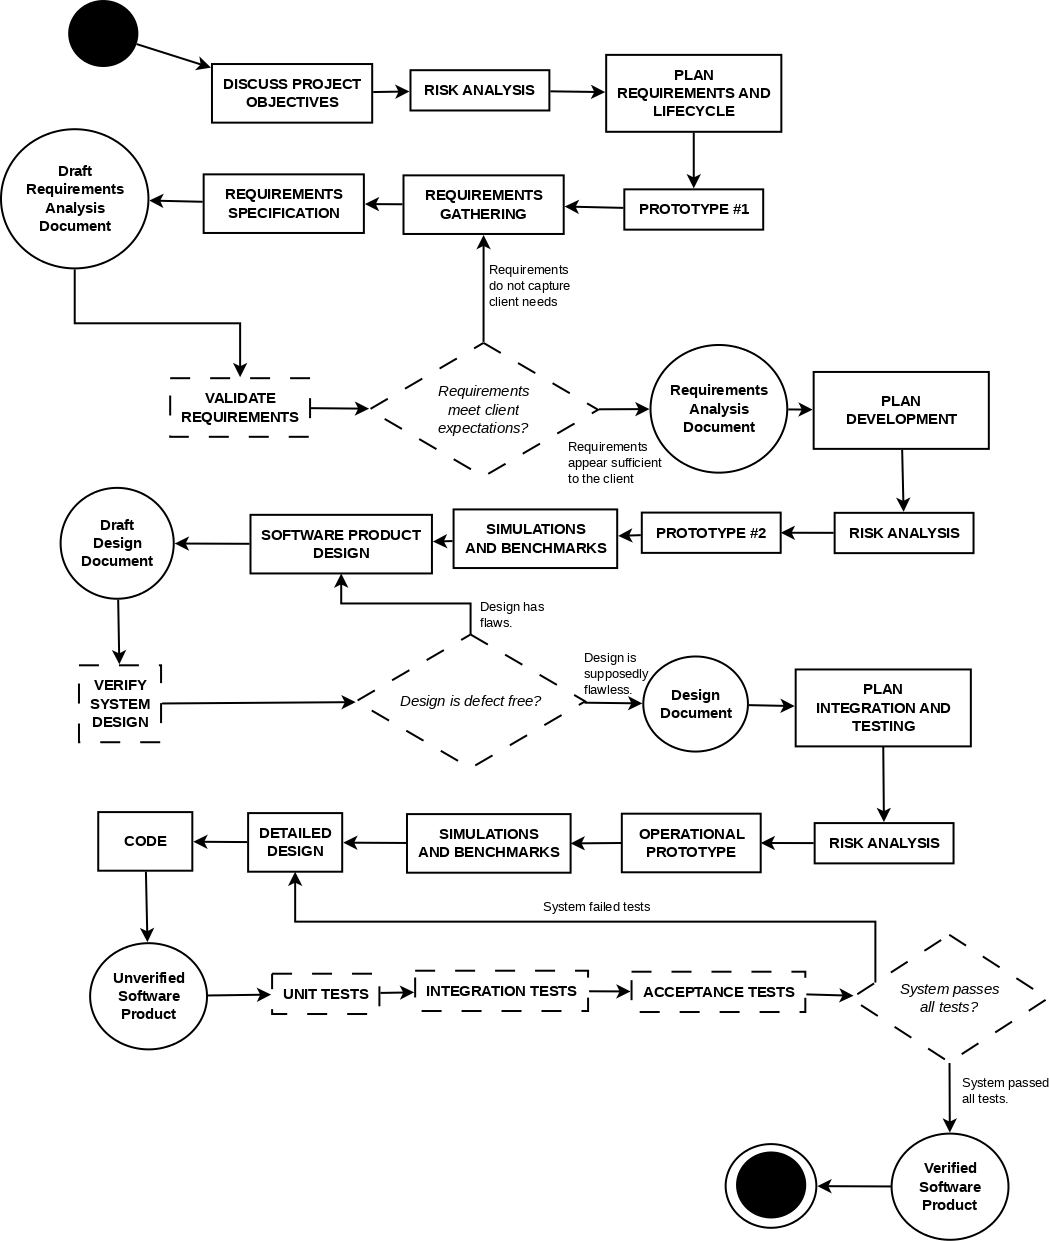
\includegraphics[scale=0.3]{media/Spiral}
	\caption{Barry Boehm's spiral model. We note that it is quite similar to Figure
		\ref{waterfallRoyceThree}.}
	\label{Spiral}
\end{figure}

In reality, this model is actually the SDLC, with more specifications, more risk analysis, and
in \cite{Boehm:1986:SMS:12944.12948} it is rolled up in a spiralling shape.
This does not change that it is really the SDLC waterfall model.
Furthermore, it is unclear in the initial paper what verification is, or where the process should go
back to when a verification point fails.
This is a weakness of the Spiral model, and the Waterfall models as well, though Boehm is more
explicit as to where backtracking should lead to when a defect is uncovered.\\
\\
The spiral model does not represent a significant shift in industry mindset and indeed, we note that
it still ascribes to the ``single stage, verifiy that everything is correct, move onto next stage"
mindset that early industry had.

\subsection{V-Model}

We note that the V-Model is perhaps one of the last of the Waterfall-esque models.
It is introduced by Fosberg et. al in \cite{forsberg1995relationship}.
Again, we note its roots in systems and ``traditional" engineering, where a stage-by-stage based
approach is taken.
Its main difference is perhaps the large amount of preparation and planning to construct plans for
verification.
These plans are constructed before project implementation, and the explicit highlighting of this
construction distinguishes SLDC from the V-model.
We show the V-Model within our notation in Figure \ref{VModel}.

\begin{figure}
	\centering
	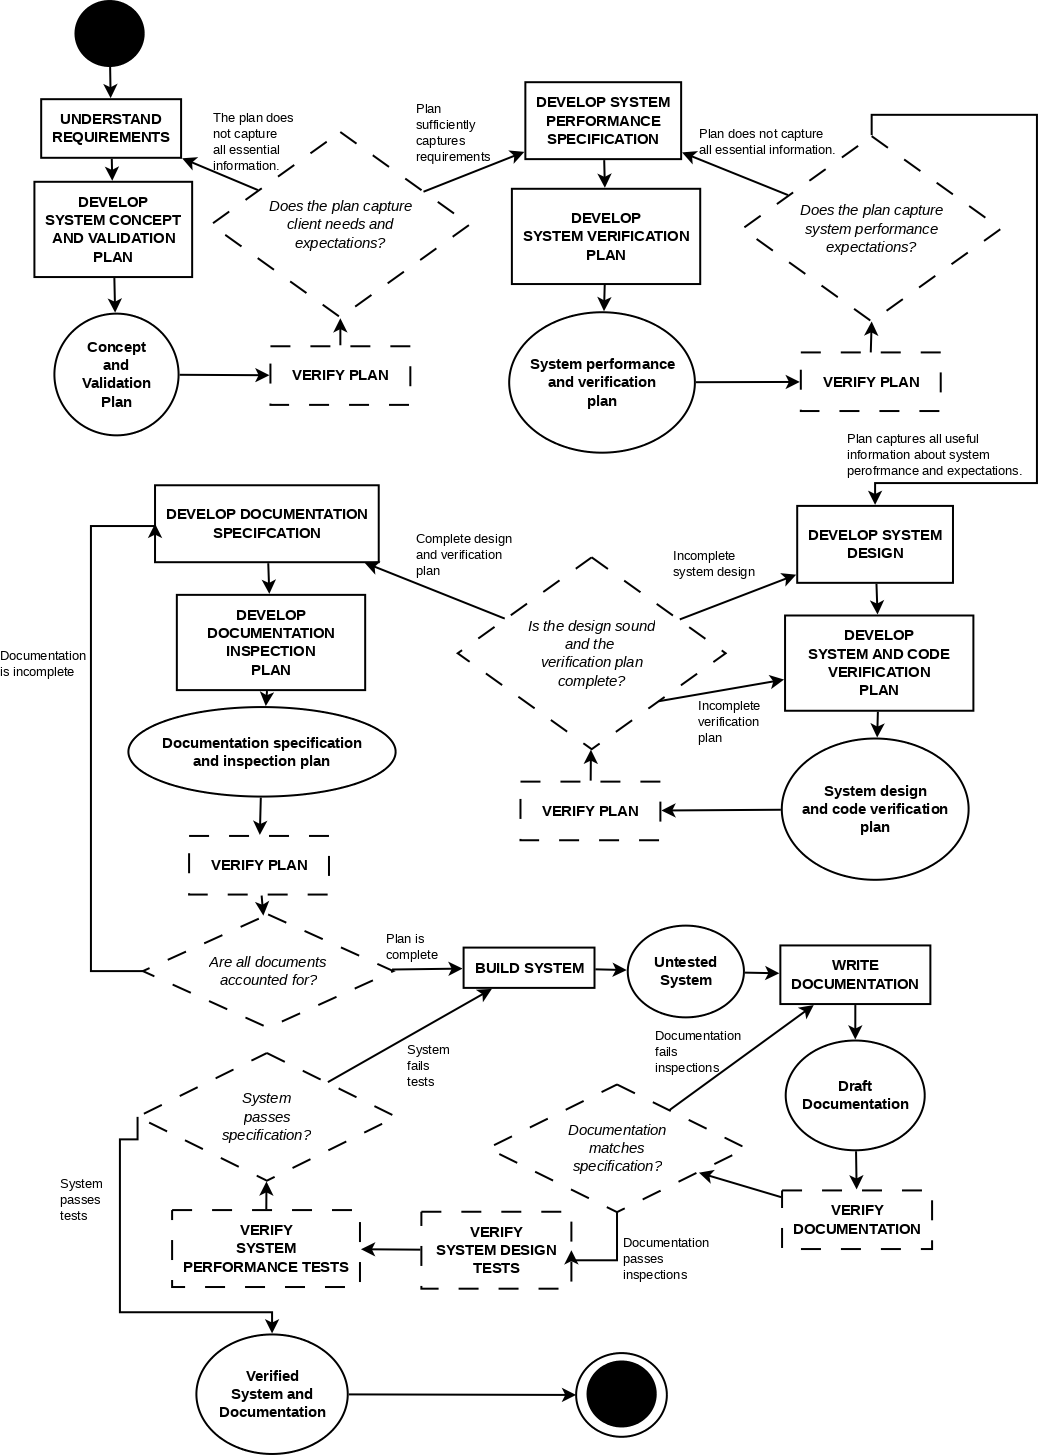
\includegraphics[scale=0.3]{media/VModel}
	\caption{The V-Model, as represented within our notation. Due to its many verification construction stages it is quite an extensive
		model within our notation. One might comment that it is a weakness of our notation that some
			models have become extremely large.}
	\label{VModel}
\end{figure}

\subsection{Rapid Prototyping}
Rapid prototyping, as was specified in \cite{Alavi:1984:APA:358080.358095}, is a process
specifically concerned with requirements gathering.
It constructs small prototypes that are mockups of the final system to assist in understanding a
client's requirements.
As a result, we will make two simplifications for our modelling of the rapid prototyping process.
\begin{enumerate}
	\item the process only changes requirements gathering, and other processes remain the same
	\item we need only model requirements gathering process, up to the generation of a requirements
	analysis document to show how rapid prototyping works
\end{enumerate}

Based on these assumptions, we show Rapid Prototyping in our own notation --- see Figure
\ref{RapidProto}. We note that this methodology would be ineffective in the case that building a prototype would be very
inexpensive or a user might not have much interaction with the system.

\begin{figure}
	\centering
	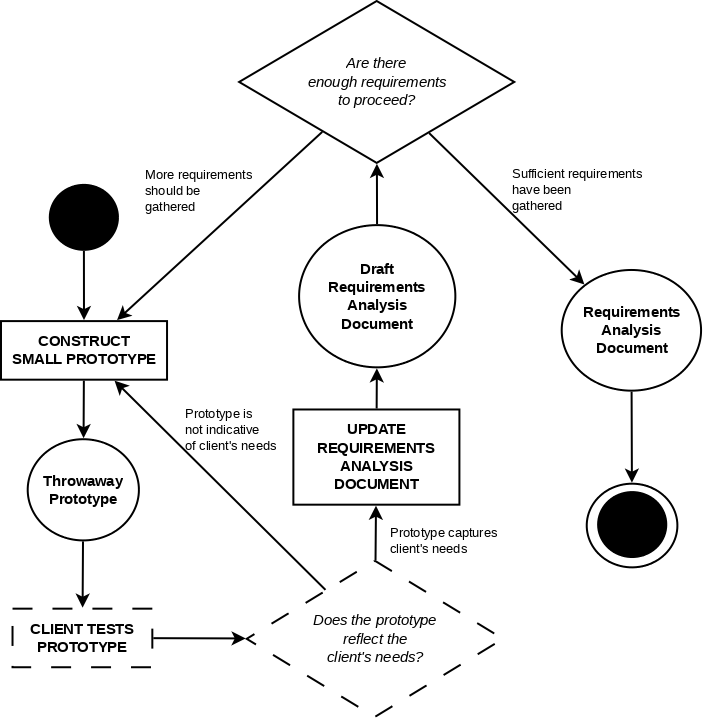
\includegraphics[scale=0.4]{media/RapidPrototyping}
	\caption{Rapid prototyping is shown above, only being used in the requirements gathering stage.
		This is also known as ``throwaway prototyping", due to the prototype being used onl in
			requirements gathering, but not in production code.}
	\label{RapidProto}
\end{figure}


\subsection{Incremental}
In \cite{pressman1992software}, Pressman suggests that an iterative, or incremental application of the
Waterfall model would be a way to offset the problems in software.
It is difficult to see much value in this mode of thinking, since it is not fine-grained enough or flexible
enough to truly make use of iteration.
It is worthwhile noting that it is difficult to see when it is appropriate to stop building or
iterating.
We provide an interpretation of this model in our own notation in Figure \ref{IncrementalFig}.

\begin{figure}
	\centering
	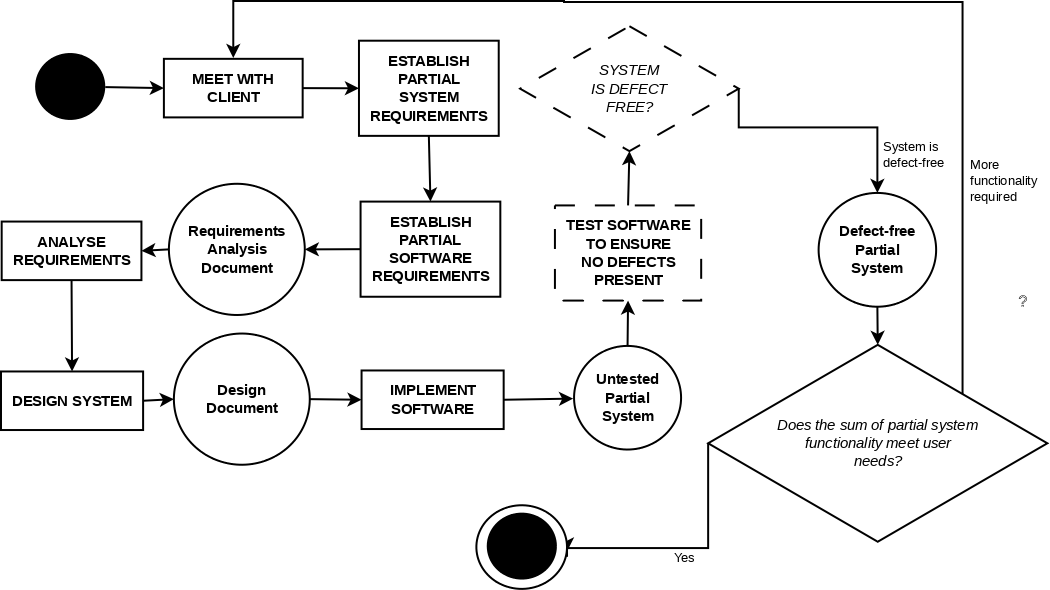
\includegraphics[scale=0.3]{media/Incremental}
	\caption{The incremental model. Our references have suggested it is merely a Waterfall model being
		applied iteratively to small chunks and we have modelled it as such.}
	\label{IncrementalFig}
\end{figure}

\subsection{Evolutionary}

We refer to the lecture given by Woodings, when we discuss Tom Gilb's evolutionary paradigm
\cite{Woodings2013Lecture2}.
In it, Woodings discusses the idea of building a house using the evolutionary paradigm, and of growing
software.
Unfortunately, we cannot actually distinguish between incremental and evolutionary within this
context.
To our mind, they might simply be the same methodology.
We again reference Figure \ref{IncrementalFig}, as there appears to be no difference in the
description of Evolutionary or Incremental software methodologies.

\subsection{Extreme Programming}
Extreme programming was first developed by Beck, and formalised in \cite{beck2004extreme}.
It is an extremely streamlined process emphasising a lot of feedback loops, and a quick turnaround.
It is noteworthy that we have come across an aspect of the process that we cannot communicate;
namely, the timely and short manner in which Extreme Programming goes about its tasks.
Beck highlights pair coding, clear communication and a quick delivery and release time as key
attributes of the extreme programming software methodology.
We outline it below in Figure \ref{WindowsXP}.

\begin{figure}
	\centering
	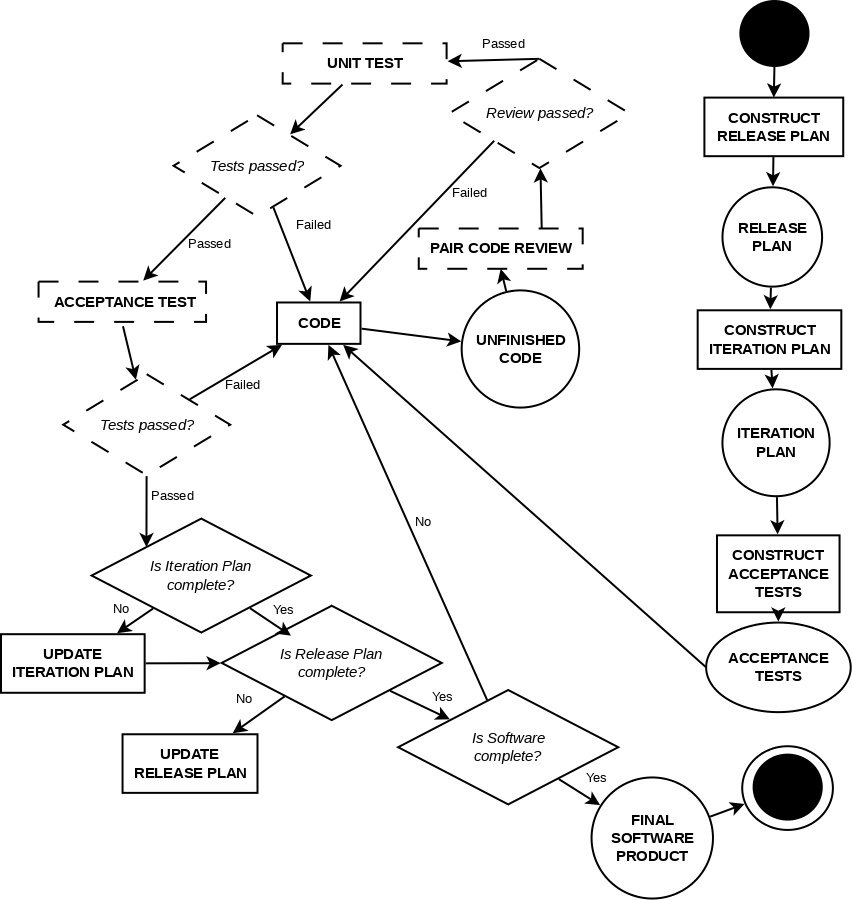
\includegraphics[scale=0.3]{media/EXP}
	\caption{The Extreme Programming methodology focuses on quick, constant feedback and short
		iterations.}
	\label{WindowsXP}
\end{figure}

\vfill
\pagebreak

\subsection{Crystal Clear}
Crystal Clear was introduced by Cockburn in \cite{cockburn2004crystal}.
He constructs a small-team methodology that particularly focuses on
\begin{itemize}
	\item frequent delivery
	\item reflective improvement
	\item osmotic communication
\end{itemize}

It stresses user involvement in the development process and has a somewhat happy union of advantages
that SDLC offers with the development process of Scrum, but with a more light-weight version of the
documentation-heavy SDLC.
We present in Figure \ref{CrystalClean} the Crystal Process in our notation.

\begin{figure}
	\centering
	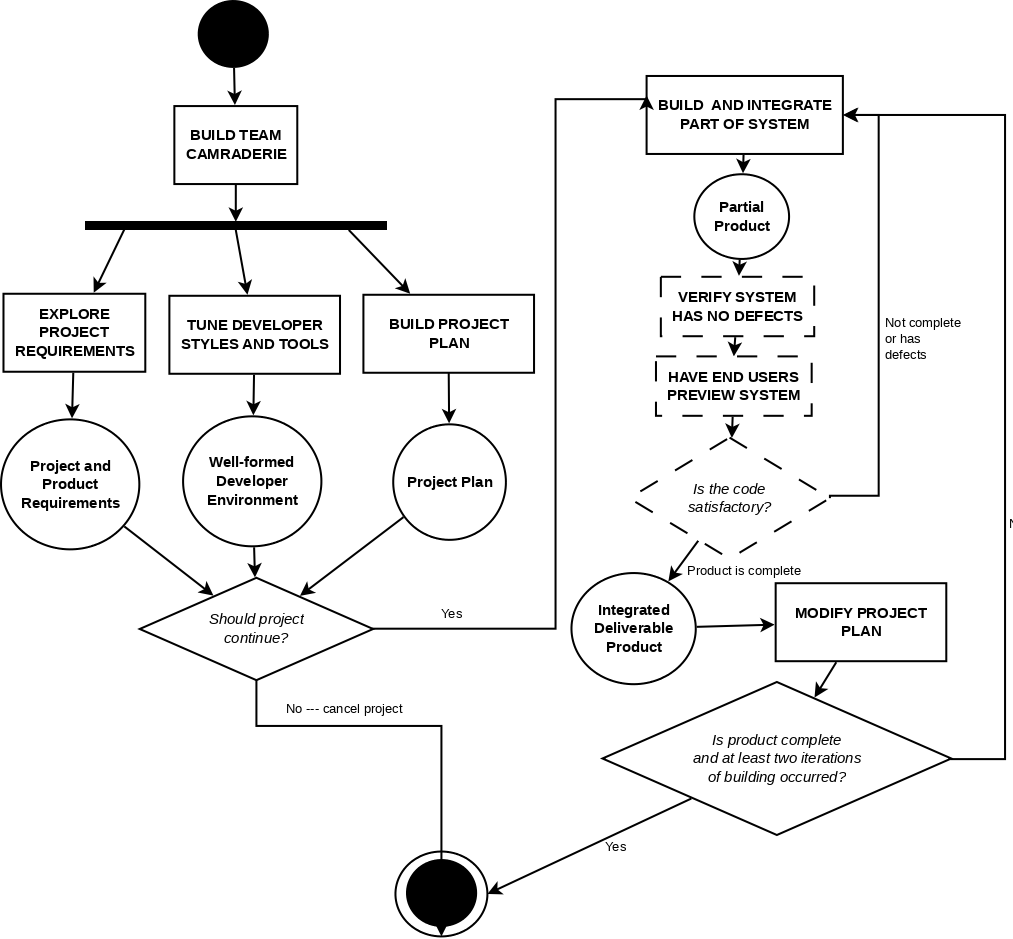
\includegraphics[scale=0.3]{media/Crystal}
	\caption{The Crystal Clear process is interesting in that it also recommends a point where the
		methodology dictates exiting and cancelling a project. This is not so clear in the other
			methodologies, and is instead implicit.}
	\label{CrystalClean}
\end{figure}

\subsection{Test-Driven Development}

Test-Driven Development was introduced and formalised by Beck in \cite{Beck:2002:TDD:579193}.
It is an interesting method that is localised to the development stages.
Primarily, it advocates writing a test and having it fail before writing the code itself.
We make the following two assumptions:
\begin{itemize}
	\item test-driven development does not influence any other tasks besides development and testing
	\item test-driven development can be fully modelled by simply looking at the development stage
\end{itemize}

We show Test-Driven Development in Figure \ref{TDD} using our notation.

\begin{figure}
	\centering
	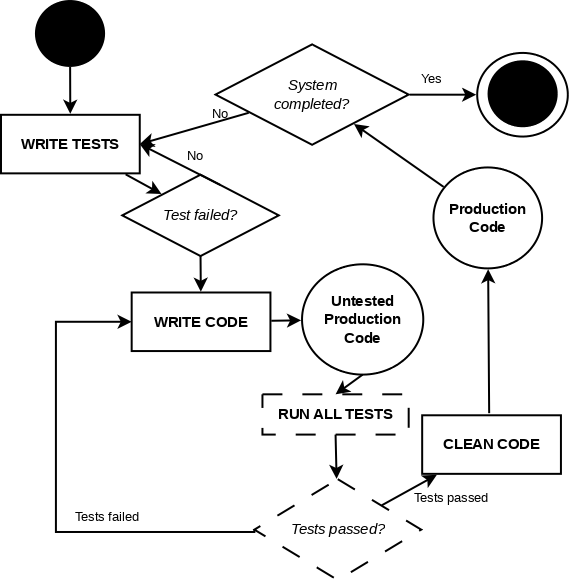
\includegraphics[scale=0.35]{media/TDD}
	\caption{Test-Driven Development is a simple method of specifying the testing strategy first, then
		the development afterwards.}
	\label{TDD}
\end{figure}

\subsection{Scrum}
The Scrum model was first introduced by Takeuchi and Nonaka in \cite{takeuchi1986new}.
This is a much more agile-like process, without as many sequential steps and many more iterative
loops and decision points.
It eschews documentation and analysis for coding and continuous design.
This would be appropriate for user-facing software that an engineer or development team is already
familiar in coding or working with.
We show a representation of the Scrum process in our own notation in Figure \ref{ScrumFig}.

\begin{figure}
	\centering
	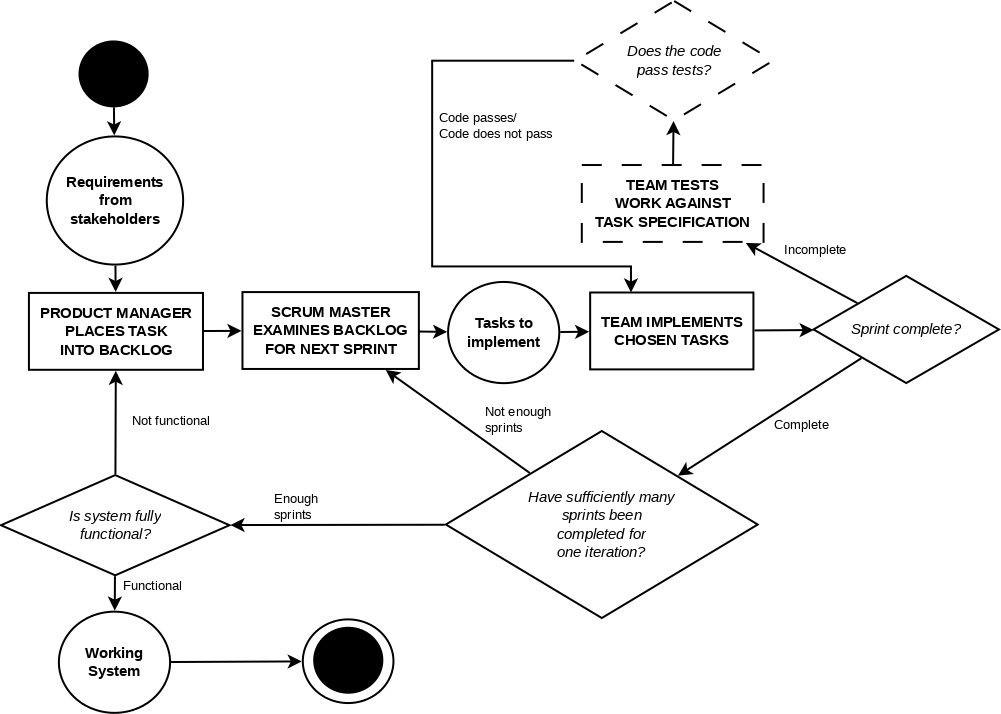
\includegraphics[scale=0.3]{media/Scrum}
	\caption{Scrum is a development model for software, and here we can see the feedback and
		simplified, easy-to-understand and responsive process that Scrum employs.}
	\label{ScrumFig}
\end{figure}

\subsection{My Process}
I also document my own process.
It bears some resemblance to Crystal Clear, but is tailored for a single-developer project where
requirements are easily understood and external verification is possible.
It concentrates on maintaining documentation so that another developer could easily join or take
over the project.
In a team environment, I would prefer to use a Scrum-like methodology or Crystal Clear pseudo-method
to encourage clear communication within the team.
My process is denoted in Figure \ref{MyProcess}.

\begin{figure}
	\centering
	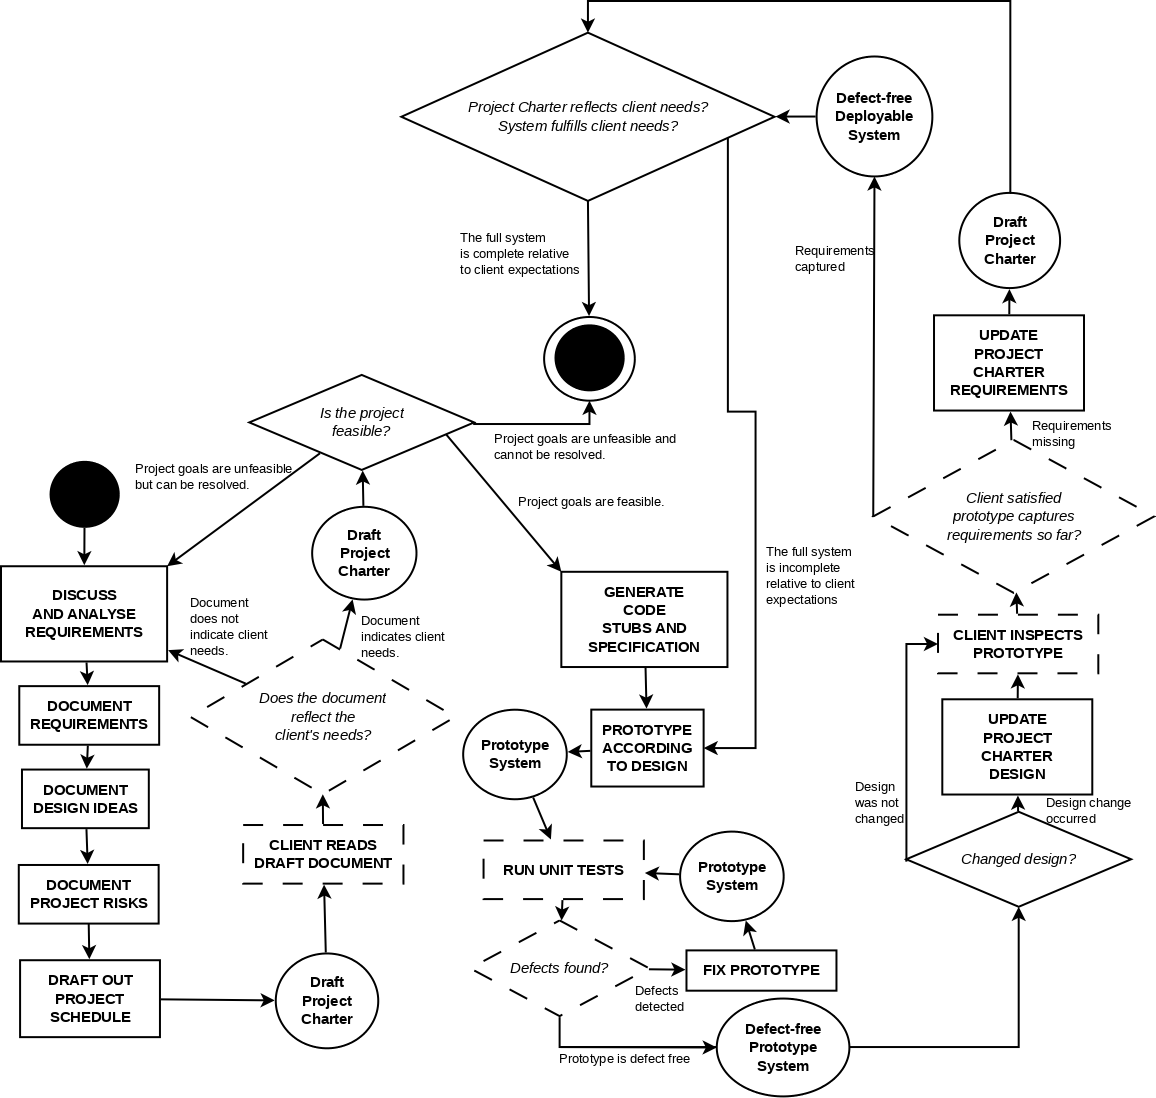
\includegraphics[scale=0.3]{media/MyProcess}
	\caption{My process; in particular, note the heavy emphasis on updating documentation of the
		project to match actual project state, and the need to ensure client input at every round of
			input. Furthermore, the similar idea from Scrum and Crystal Clear --- that the client is
			delivered working code on a timely, continuous basis.}
	\label{MyProcess}
\end{figure}

\section{Software Taxonomy} \label{taxonomy}

In \cite{Woodings2013Tut1}, Woodings displays an example taxonomy in the form of
a decision tree.
We aim to replicate the decision tree hierarchy by noting some interesting
structural and semantic differences between the models and thus be able to
comment on the interesting and salient characteristics of each.\\
\\
We begin by noting that there are ``iterative" and ``non-iterative" models.
But what does this actually mean?
Many of the processes we made in our notation have a ``verification" stage that
iterates within the stage.
``Iterative" and ``non-iterative" are thus too general labels to begin with.\\
\\
Instead, we note that the ``agile" and ``non-agile" methods have two very
different features.
``Agile" methods have feedback from clients and users during the coding stage as
to how the product so far looks.
``Non-agile" methods do not engage in this; they specify requirements at the
beginning, get them as correct as possible, and then continue with the
implementation.\\
\\
We can thus use a first division as {\bf ``does the process have a user-feedback
stage during implementation?"}
This almost neatly divides our set of models in two partitions, $S_{yes}$ and
$S_{no}$ (for ``yes" and ``no" to our answer respectively).
The ``evident" partitions would be
\begin{itemize}
  \item $S_{yes} = \{$ Crystal Clear, Extreme Programming, Evolutionary, Scrum $\}$
  \item $S_{no} = \{$ Waterfall-1, Waterfall-2, Waterfall-3, Spiral, V-Model$\}$
\end{itemize}
There are three interesting cases that are more difficult to classify
\begin{enumerate}
  \item the incremental model is an iterative, semi-agile model that revolves
  around implementing small chunks of work in a waterfall-esque fashion.\\
  \\
  One might argue that a single iteration of waterfall is an implementation stage,
  but we will choose to instead say that the implementation or coding stage of
  the waterfall iteration is the task which needs a user-feedback stage.\\
  \\
  As it does not, we can say that it is belongs in the $S_{no}$ partition.
  \item similarly, test-driven development is another interesting case due to
  its iterative nature.
  However, pure test-driven development does not contain a user-feedback stage,
  and it is a simple methodology to encode a testing mindset into developers.
  As a result, we say that test-driven development also belongs in $S_{no}$.
  \item rapid prototyping does not actually revolove around the implementation
  stage, since it is a special case of requirements gathering.
  Since by our original modelling assumptions, this requirements gathering is
  independent of any other process in the development methodology, rapid
  prototyping does not belong to $S_{no}$ or $S_{yes}$.\\
  \\
  Instead, we create a third partition, $S_{rapid} = \{$ Rapid Prototyping $\}$ which is a singleton set
  containing only rapid prototyping.
\end{enumerate}

So far, we have divided our initial set of models into three possible models.
This is shown in Figure \ref{DecTree1}.

\begin{figure}[ht!]
  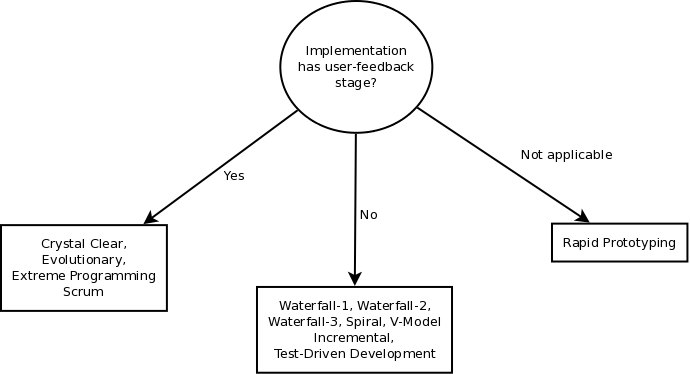
\includegraphics[scale=0.4]{media/DecisionTree1}
  \caption{Our initial decision tree. We can see each of $S_{no}$, $S_{yes}$ and $S_{rapid}$.}
  \label{DecTree1}
\end{figure}

We will focus on subdividing $S_{yes}$.
These are models that are ``agile" in their mannerisms.
We note that out of the four models, two of them involve modifying a project
plan.
The others do not; instead, both Scrum and Evolutionary are feature-driven, with
an intent to ``grow" the project (indeed, we might find they are the same
process by the end!).
We will thus subdivide $S_{yes}$ into two new partitions
\begin{itemize}
  \item $S_{plan} = \{$ Crystal Clear, Extreme Programming $\}$
  \item $S_{grow} = \{$ Scrum, Evolutionary $\}$
\end{itemize}
This labelling reflects some interesting properties of the methods under review.
We note that the two partitions are focused on an organic method of
growing a project, versus a prescribed plan that should be flexible when meeting
user requirements.
Both of these are in the spirit of ``user-feedback" and ``user-focused"
development, but one might have more group might have more foresight and risk
management inbuilt ($S_{plan}$) whilst the other might be more flexible and
reactive ($S_{grow}$).\\
\\
We have achieved a further level of granularity with our second subdivision.
This is shown in Figure \ref{DecTree2}.
\begin{figure}[ht!]
  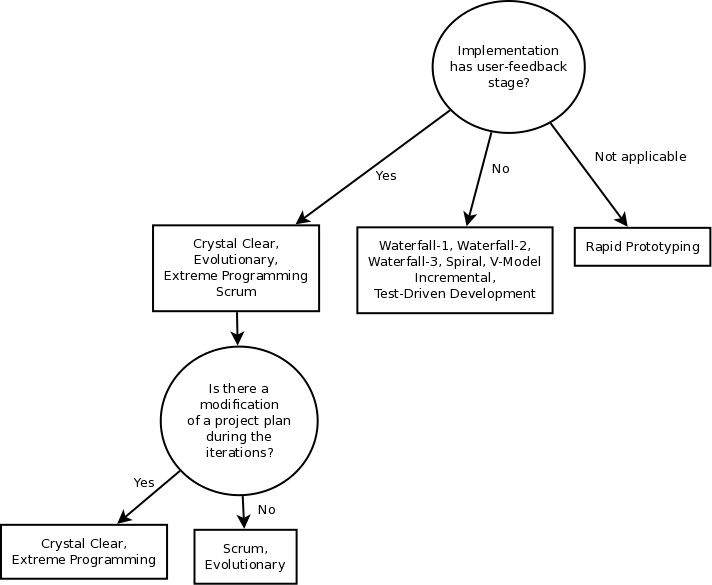
\includegraphics[scale=0.4]{media/DecisionTree2}
  \caption{A second iteration of our decision tree. We have now managed to
  subdivide $S_{yes}$ into sets of size two.}
  \label{DecTree2}
\end{figure}

We now find some interesting results.
When trying to separate Scrum and Evolutionary, it becomes difficult to find
many differences between the two.
Perhaps the only real differences lie in the meanings behind what happens; there
are assigned roles in Scrum for studying and deciding what users want, whereas
Evolutionary does not have as rigid structure in organising the system.
We will use this to differentiate between the two processes, though we note that
this is a small difference and it is hard to justify this as a good
differentiator between the two.\\
\\
To separate Extreme Programming and Crystal Clear, we note that in Figure
\ref{WindowsXP} there is a mandatory requirement of Peer Review and Pair Coding.
The verification process in Crystal Clear does not have nearly so many levels of
verification around coding specified.
Thus, we use the following question as our discriminator: ``are there multiple
levels of verification centred around coding specified in the process?"\\
\\
We should note that the questions at this level are very subjective and are not
as definitive as our previous questions.
As an example, the testing process in Crystal Clear is not specified; a
practitioner could add in multiple feedback loops and thus almost make it
indistinguishable from Extreme Programming.
Thus, in some cases, we could claim that Extreme Programming and Crystal Clear are the
same process, and the same could be said of Scrum and Evolutionary.
Thus, we will use a dotted line to represent a pseudo-``equivalence class" of
processes that are almost the same, except for perhaps some implementation
differences.
Figure \ref{DecTree3} is our first iteration of actual definitive classification
(that is, we can now actually classify some models based on their
characteristics).

\begin{figure}[ht!]
  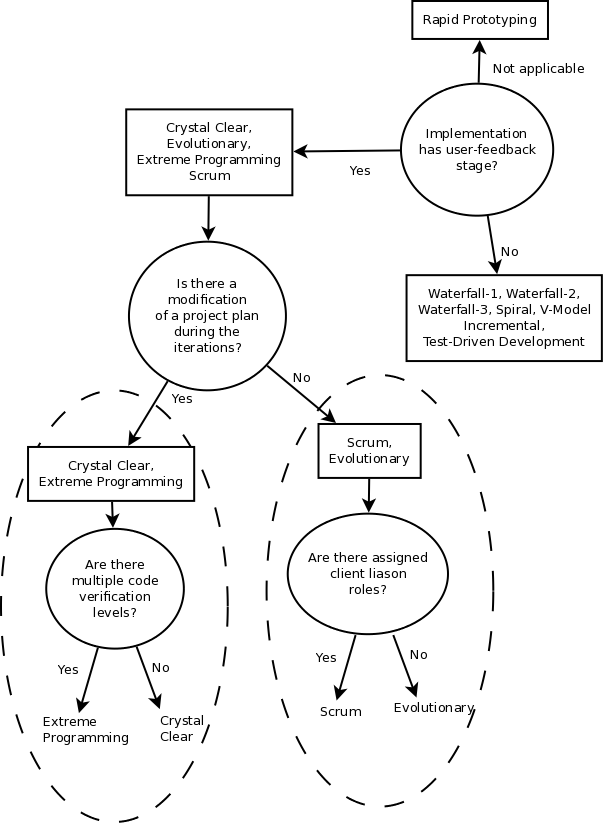
\includegraphics[scale=0.4]{media/DecisionTree3}
  \caption{A third iteration of our decision tree. We can definitively classify
  four of our processes by their structure and semantics, and we use an
  ``equivalence class" to denote models that appear to be the same.}
  \label{DecTree3}
\end{figure}

We now consider the problem of subdividing the much larger class $S_{no}$ into
partitions.
We note the following unique characteristics
\begin{itemize}
  \item Waterfall-1 has no feedback at all
  \item Waterfall-2 and Waterfall-3 have iterations between stages
  \item Test-Driven Development is only a specification of how to write code
  during the implementation stage
  \item Incremental is an iterative loop methodology
  \item Spiral has a risk-assessment stage inbuilt into the project
  \item V-Model specifies all verification plans before the implementation
  begins
\end{itemize}

These are definitive characteristics in our notation and we will use them to
subdivide $S_{no}$.
Of note is that these questions or defining characteristics are in many cases
ambiguous; having a risk-assessment stage is something that could be easily
built into another process, and it is thus difficult to at times distinguish
between models.
Refer to Figure \ref{DecTree4} for our breakdown of models.
For compactness, we only show the subtree of our decision tree that breaks down
$S_{no}$.

\begin{figure}[ht!]
  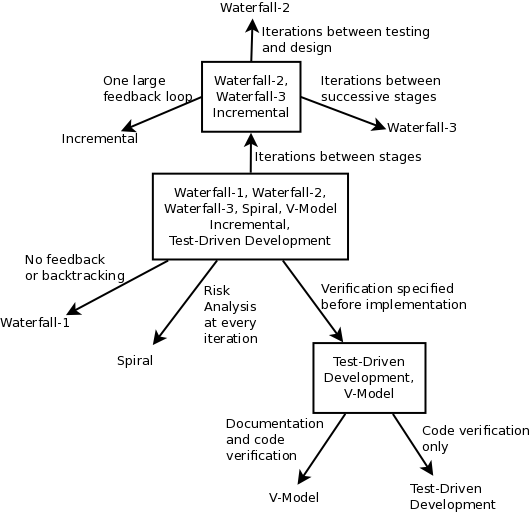
\includegraphics[scale=0.4]{media/DecisionTree4}
  \caption{This showcases the classification scheme for the models in $S_{no}$.
  We use a compressed form to show the classification of each of the models.}
  \label{DecTree4}
\end{figure}

We show a final decision tree that shows our classification scheme for each of
the models in Figure \ref{DecTreeFinal}.
It is by no means the definitive standard, and indeed it has flaws that we will
explore in the next chapter.
It serves as a baseline that could perhaps later be improved.

\begin{figure}[ht!]
  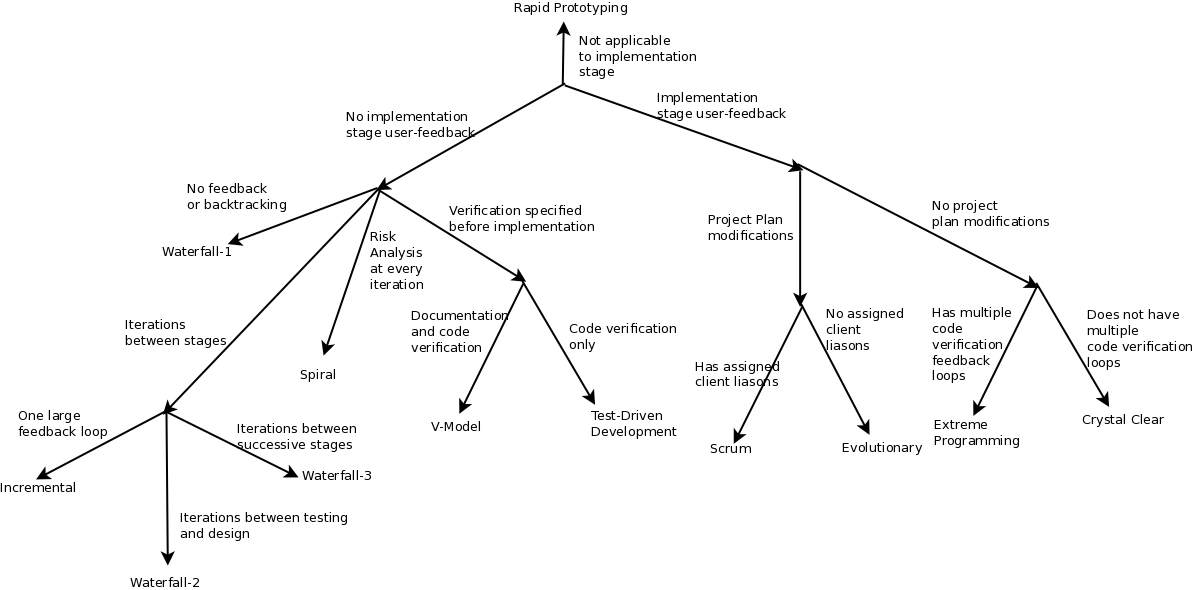
\includegraphics[angle=90,scale=0.35]{media/DecisionTreeFinal}
  \caption{Our final decision tree that we have induced. We comment on its
  accuracy, usefulness and lessons learnt in the next chapter.}
  \label{DecTreeFinal}
\end{figure}

As a last exercise, we ask ourselves where my process would go.
During implementation, there is a definite client-verification stage.
Furthermore, there is the modification of the project charter, which itself
contains a project plan and requirements.
Lastly, there is only one code verification stage in my process; this suggests
that my process is an implementation of Crystal Clear.
This identifies a weakness in my taxonomy, as Crystal Clear is a team-based
methodology.
We discuss this in the next chapter.

\begin{A Taxonomy for Projects}

Unfortunately, we are left with insufficient time to truly explore the second
question; a taxonomy for projects to map them to appropriate processes.
We note the following
\begin{itemize}
  \item a safety critical system would benefit from the Spiral or V-Models, due
  to their concentration on risk mitigation and solid verification criteria
  \item scientific or batch programs that are not user facing will {\em not}
  find much benefit from processes where user-involvement is requried; that is I
  believe that Crystal Clear, Extreme Programming, Scrum and Evolutionary
  methods are inappropriate for non-user facing systems
  \item conversely, high end-user interaction where requirements are extremely
  dynamic are almost certainly better off using any of Crystal Clear, Extreme
  Programming, Scrum or Evolutionary methods
\end{itemize}

Yet these are rudimentary comments.
They are not a taxonomy unto themselves, and are self-evident from the Agile and
SDLC philosophies and approaches to Software Development.
I leave it as future work and an open question to address how to effectively
select a software development methodology given a set of requirements.

\section{Analysis} \label{secAnalysis}

With our results in hand, we now return to our seven questions we outlined in
section \ref{secMethod}.
Using our results we will answer each of them and comment on any insights we
have.

\subsection{Question one}

Originally, we wanted to know
\begin{quote}
  To what extent does learning carry over between two software projects of similar
  specifications?
\end{quote}
And, within our experimental framework we translated this to 
\begin{quote}
  What are the differences in $a$ between \PO\ using \LA\ and \PT\ using \LA?
\end{quote}

Our values for $a$ from our best fits for \PO\ using \LA\ and \PT\ using \LA are
shown in Tables \ref{table:P1LA:abc} and \ref{table:P2LA:abc} respectively.
We aggregate them and find that
\begin{itemize}
  \item the average of $a$ in \PO\ using \LA\ is 172.6738 minutes
  \item the standard deviation of our $a$ parameters in \PO\ using \LA\ is 0.23896 
  \item the average of $a$ in \PT\ using \LA\ is 100.0073 minutes
  \item the standard deviation of our $a$ parameters in \PT\ using \LA\ is
  0.068343
\end{itemize}

These low standard deviations suggests that these are very accurate estimates on
the amount of time a student takes to finish off a problem with no information
or knowledge about it.
This is sensible since the $a$ values were all very similar, and each model
should have started off with the same result for the first attempt at finishing
the problems.\\
\\
We note that between the \PO\ in \LA\ and \PT\ in \LA, there was a 72 minute
drop.
This is equivalent to a $42\%$ decrease in the required time to complete the
task, relative to the time taken in \PO\ in \LA.
It seems sensible that knowledge and time taken are inversely correlated.
Our results suggest that after completing a similar task, there is an increase of
$42\%$ in knowledge which is usable for this similar task.
Obviously, this is not entirely true --- there are differences in the tasks we
are using that we have not empirically considered.
Furthermore, we do not have a baseline of solving \PT\ without any prior
knowledge, but this gives an initial estimate on the increase of knowledge.

\subsection{Question two}

Our original question two asked
\begin{quote}
  To what extent does learning carry over between two software projects using
  similar resources?
\end{quote}

Within our experimental framework, this question asked
\begin{quote}
   What are the differences in $a$ between \PO\ using \LA\ and \PO\ using
  \LB?
\end{quote}

Again, we aggregate the $a$ values shown in Table \ref{table:P1LB:abc} and find
that
\begin{itemize}
  \item the average of the $a$ values of \PO\ using \LB\ is 102.9797 minutes
  \item the standard deviation of the $a$ values for \PO\ using \LB\ is 0.655761
\end{itemize}

The drop in $a$ values --- that is, the difference between the mean for \PO\
using \LA\ and \PO\ using \LB\ is very similar to what we found for Question
One.
Indeed, this is a 70 minute decrease, from the initial attempt in \PO\ in \LA\
to the first attempt for \PO\ in \LB.
This is a $40\%$ decrease compared to the $a$ value in \PO\ in \LA, and is quite
comparable to the decrease in the $a$ value in the previous section (\AZ\ of
\PO\ in \LA\ to \AZ\ of \PT\ in \LA).\\
\\
I had a personal suspicion that a language change would have a more significant
increase in knowledge and decrease in time than a change in problem
specification but our results suggest otherwise.
However, I do not think our results are conclusive and might actually support my
suspicions since prior to solving \PT, the students had actually completed \PO\
(a similar problem) problem eight times.
Conversely, when completing \PO\ in \LB\ they had only completed \PO\ four times.
This anomaly in process and experimental methodology suggests that
there is scope for more investigation and that my suspcions should not be
discarded yet.

\subsection{Question three}

Question three originally asks
\begin{quote}
  To what extent does practice enable us to better predict the effort required
  for software?
\end{quote}

This translates to us asking
\begin{quote}
  How well do our models fit the data?
\end{quote}

We want to know whether practice gives us better fits of models --- better fits
will suggest that our models are more useful for later predictions.
To answer this question, we will compare the sum of squares of the three
different datasets.
These are summarised in Tables \ref{table:P1LA:abc:sumsquares},
\ref{table:P1LB:abc:sumsquares} and \ref{table:P2LA:abc:sumsquares}.
We notice that \PO\ using \LA\ gives nonsensical results, and in fact our models
were inappropriate for actually doing much prediction (besides, perhaps $m_3$).
However, in \PT\ using \LA\ and \PO\ using \LB\ we retrieved sensible and useful
results.
\PO\ using \LB\ in particular had very good fits overall, with low sums of least
squares.\\
\\
I believe that this is due to actually practicing more on the same problem ---
we note that after performing the same problem (\PO) multiple times, even in
different languages, gives a more predictable result and is easier to fit a
model to.
Conversely, even though the problem is similar, the learning rate is much more
erratic and difficult to fit when completing \PT, despite using \LA.
This suggests that practicing on the same problem, regardless of language, will give more
consistent and predictable results for modelling purposes, whilst different
problems will cause issues with regards to being able to fit a model.

\subsection{Question four}

Our original question four asks
\begin{quote}
  How does learning differ as we practice on different problems? 
\end{quote}

We translate this, within the framework of our experiment to
\begin{quote}
   How does $b$ change between each of \PO\ in \LA, \PO\ in
   \LB\ and \PT\ in \LA?
\end{quote}

We resummarise all the $b$ results from each dataset, for each model in Table
\ref{table:beees}.

\begin{table}[ht!]
\centering
\begin{tabular}{|c|c|c|c|}
\hline
  & $m_1$ & $m_2$ & $m_3$ \\
\hline
\PO\ in \LA & N/A & N/A & 0.794716 \\
\hline
\PO\ in \LB & 1.05646 & 1.05789 & 1.03095 \\
\hline
\PT\ in \LA & 1.78221 & 1.62075 & 1.39094 \\
\hline
\end{tabular}
\caption{These are the $b$ values from each fit. We omit the unreliable results
for $b$ in $m_1$ and $m_2$ for \PO\ in \LA.}
\label{table:beees}
\end{table}

There is an overall trend of $b$ increasing as the students do more iterations.
We ought to note that the $b$ value increasing makes the curve steeper, and it
reaches its horizontal asymptote (the value for $c$) much more quickly.
This suggests that reinforcement of knowledge through practice increases
learning and is an observable phenomena.\\
\\
An interesting question to ask is if the learning itself is asymptotic.
How much practice could we do before we would not increase learning anymore?
Figure \ref{fig:BvalueFit} is a graph showing the means of the $b$ values and
the overall trend polynomial trend.

\begin{figure}[ht!]
\centering
\FIXME
\caption{The $b$-values after aggregation between each dataset.}
\label{fig:Bvaluefit}
\end{figure}

I think that we do not have enough data to make a conclusive comment about this,
but it is important to note that at present, the learning value apparently
is unbounded, and furthermore increases at an unbounded rate (by taking the
derivative of the equation of best fit).
This seems nonsensical to me, and I would suggest doing further analyses beyond
this rudimentary inspection to determine how learning changes and how learning
itself is affected between each iteration.

\section{Conclusion}

% Every research paper should answer the following questions:
% 
% \begin{itemize}
% \item What did you do?
% \item Why did you do it?
% \item What happened?
% \item What do the results mean?
% \item What is your work good for?
% \end{itemize}
% 
% Make sure that your conclusion leaves the reader with the answers
% to these questions clearly in mind.
% 


% appendices

\bibliographystyle{ieeetr}
\bibliography{assignOne}

\end{document}
